\section{Research method}\label{sec:research_method}
This section describes the research method used in this mapping review for identifying and analyzing relevant papers. It is mainly based on the software engineering systematic literature review guidelines and recommendations proposed by Kitchenham et al.~\cite{Kitchenham:2007}, Brhel et al.~\cite{Brhel:2015}, Souza et al.~\cite{Desouza:2015}, and Petersen et al.~\cite{Petersen:2008}. These authors suggest a process with three main steps: planning, conducting, and reporting. In the planning step, they recommend defining a review protocol that includes a set of research questions, inclusion and exclusion criteria, sources of papers, search string, and mapping procedures. In the conducting step, they recommend selecting and retrieving papers for data extraction. Finally, in the reporting step, they recommend analyzing the results used to address research questions defined before.

\subsection{Research questions}\label{subsec:questions}
The main goal of this mapping review is to provide a current status of the research on bug report severity prediction in FLOSS. To ensure an unbiased selection process, this review addresses the following research questions.

\begin{enumerate}[label=\textbf{ RQ$_{\arabic*}$}., leftmargin=1.2cm]
  %% RQ1
  \item \textbf{When and where have the studies been published?} This research question gives to the researcher a perception whether the topic of this mapping review seems to be broad and new, providing an overview about where and when papers were published.
  
  %% RQ2
  \item \textbf{What FLOSS are the most used as report sources in experiments for bug report severity prediction?} This research question names the FLOSS used as report source in problems of bug report severity prediction. This overview can be useful for researchers that intend to accomplish new initiatives in this area, and can also motivate the adoption of new FLOSS in future research to bridge existing gaps.
  
  %% RQ3
  \item \textbf{Was bug report severity prediction most addressed as either a fine-grained label  or coarse-grained label prediction problem?} This research question investigates whether bug report severity prediction was handled as a fine-grained label (i.e., multi-label) or as a coarse-grained label (i.e., two-label or three-label) prediction problem. Understanding each solution provided for each prediction problem type is essential for guiding the selection of suitable machine learning algorithm.
  
  %% RQ4
  \item \textbf{What are the most common features used for bug report severity prediction?} This question investigates features used for bug report severity prediction in FLOSS. It can help to map which features have been considered more effective for this prediction problem.
  
  %% RQ5
  \item \textbf{What are the most common feature selection methods used for bug report severity prediction?} This question complements the previous one, looking for feature selection methods employed in the papers for bug report severity prediction in FLOSS. Also, this RQ allows for identifying which feature selection approaches have been considered more suitable for this prediction problem.
  
  %% RQ6
  \item \textbf{What are the most used text mining or information retrieval methods for bug report severity prediction?} This research question indicates the main text mining approaches used to extract features from textual fields of bug reports. It can guide researchers in the task of selecting text mining methods more suitable to be applied in bug report severity prediction or similar problems. 
  
  %% RQ7    
  \item \textbf{What are the most used machine learning algorithms for bug report severity prediction?} This research question aims to identify the main ML algorithms, which have been adopted for bug report severity prediction in FLOSS. Also, this RQ can be useful for any researcher that intends to accomplish further initiatives in this area, as well as to guide him/her in search of other algorithms to advance the state of the art.
  
  %% RQ8
  \item \textbf{What are the measures typically used to evaluate ML algorithms performance for bug report severity prediction?} This research question aims to find out which measures are used to evaluate ML algorithms performance. It can be helpful to identify the more appropriate measures to evaluate ML algorithms performance for bug report severity prediction. 
  
  %% RQ9   
  \item \textbf{Which sampling techniques are applied most frequently to generate more reliable predictive performance estimates in severity prediction of a bug report?} This question complements the previous one, investigating sampling techniques, which have been used to generate more reliable and accurate ML models. It can be useful to analyze sampling techniques, which might be more suitable to improve machine learning algorithms performance for bug report severity prediction.
  
  %% RQ10
  \item \textbf{Which statistical tests were used to compare the performance between two or more ML algorithms for bug report severity prediction?} The answer to this research question can be useful to identify which statistical tests were used in the context of bug report severity prediction. In addition, it allows grasping existing protocols for the comparison between two or more ML algorithms performance using statistical significance tests.
  
  %% RQ11 
  \item \textbf{Which software tools were used to run experiments for bug report severity prediction?} This research question highlights the software tools most used to run experiments for bug reports severity prediction in FLOSS projects. It is useful to provide information for researchers and practitioners about technologies that could be used in their experiments.
  
  %% RQ12
  \item \textbf{Which solution types were proposed for the problem of bug report severity prediction?} This research question examines whether the most common solutions proposed in the selected studies are either online or off-line. This is important to separate the solutions that can be applied only in an experimental environment (off-line) from those that also can be deployed in a real scenario (online).
\end{enumerate}

\subsection{Paper selection}\label{subsec:selection}
This section describes the selection process carried out through this systematic mapping review. It comprises four steps: (i) terms and searching string; (ii) sources for searching; (iii) inclusion and exclusion criteria; and (iv) data storage procedures.

\subsubsection{Terms and search string}\label{subsubsec:string}
The base string was constructed from three main search terms related to three distinct knowledge areas: ``open source project", ``bug report" and ``severity predict." To build the search string, terms were combined with ``AND" connectors. The search string syntax was adapted according to particularities of each source (e.g., wildcards, connectors, apostrophes, and quotation marks) before it has been applied on three metadata papers: title, abstract, and keywords. Table~\ref{tab:search_string} exhibits terms and final search string used in this systematic mapping review.

\begin{table*}[ht!]
  \centering
  \spacebtrows{1.3}
  \caption{Search string.}
  \begin{tabular}{@{}ll@{}} 
    \toprule
    \textbf{Area} & \textbf{Search term}\\ 
    \midrule
    Bug report & ``bug report"\\ 
    Open source & ``open source software" \\
    Severity prediction & ``severity predict"\\ 
    \midrule
    \textbf{Search string}: & ``open source software" AND ``severity predict" AND ``bug report"\\ 
    \bottomrule
  \end{tabular}
  \label{tab:search_string}
\end{table*}

\subsubsection{Sources}\label{subsubsec:sources}
To accomplish this systematic mapping review, four electronic databases and one popular search engines were selected, as recommended by Kitchenham et al.~\cite{Kitchenham:2007}. Table~\ref{tab:search_sources} shows each selected search sources, as well as the search date, and the period covered by the search. 

\begin{table*}[!htbp]
  \centering
  %\spacebtrows{1.3}
  \caption{Search sources.}
  \begin{tabular}{@{}lllll@{}} 
    \toprule
    \textbf{Source} & \textbf{Electronic address} & \textbf{Type} & \textbf{Search Date} & \textbf{Years covered}\\ 
    \midrule
    ACM              &  \url{http://dl.acm.og}     & Digital library   & Dec,17 & 2010 - 2017\\ 
    IEEE             &  \url{http://ieeexplore.ieee.org}               & Digital library   & Dec,17 & 2010 - 2017\\ 
    Google Scholar   &  \url{http://www.scholar.google.com}  & Search engine     & Dec,17 & 2010 - 2017\\ 
    Science Direct   &  \url{http://www.sciencedirect.com}   & Digital library   & Dec,17 & 2010 - 2017\\
    SpringLink       &  \url{http://www.springerlink.com}    & Digital library   & Dec,17 & 2010 - 2017\\
    \bottomrule
  \end{tabular}
  \label{tab:search_sources}
\end{table*}

\subsubsection{Inclusion and exclusion criteria}\label{subsubsec:criteria}
The inclusion criteria below allow the identification of papers in the existing literature.

\begin{center}
  \begin{enumerate}[label=\textbf{ IC$_\arabic*$}., leftmargin=1.1cm]
    \item The paper discusses bug report severity prediction in FLOSS projects.
  \end{enumerate}
\end{center}

On the contrary, the following exclusion criteria allow excluding all papers that satisfy any of them.

\begin{enumerate}[label=\textbf{ EC$_\arabic*$}., leftmargin=1.1cm]
  \item The paper does not have an abstract;
  \item The paper is just published as an abstract;
  \item The paper is written in a language other than English;
  \item The paper is not a primary paper (e.g., keynotes);
  \item The paper is not accessible on the Web;
\end{enumerate}

\subsubsection{Data storage}\label{subsubsec:storage}
The data extracted in the searching phase were stored into a spreadsheet that recorded all relevant details from selected papers. This spreadsheet supported classification and analysis procedures throughout this systematic mapping review.

\subsubsection{Assessment}\label{subsubsec:assessment}
According to Kitchenham et al.~\cite{Kitchenham:2007}, the consistency of the protocol utilized in a systematic mapping  should be reviewed to confirm that: ``the search strings, constructed interactively, derived from the research questions";  ``the data to be extracted will properly address the research question(s)"; ``the data analysis procedure is appropriate to answer the research questions". In this research, the first author is a Ph.D. candidate running the experiments. The second and third authors conducted the review process.

\subsection{Data extraction and synthesis}\label{subsec:extraction}

Figure~\ref{fig:smr_selection_phases} illustrates the four-stage selection process carried out in the current mapping review. In each stage, the sample size was reduced based on the inclusion and exclusion criteria. In the first stage, relevant papers were retrieved by querying the databases with the search string presented in Table~\ref{tab:search_string}. All database queries were issued in December 2017. This yielded a total of 54 initial papers: 13 from \textbf{IEEE Xplore}, 5 from \textbf{Science Direct}, 17 from \textbf{ACM Digital Library}, and 19 from \textbf{SpringerLink}. After removing four duplicates, we reduced (around 7\%) the initial set of 50 papers. 
In the second stage, inclusion and exclusion criteria were applied over title, abstract, and keywords, reaching a set of 18 papers (reduction around 64\%): 32 papers were rejected for not satisfying IC$_{1}$ (The paper discusses severity prediction of bug reports in FLOSS projects). In the third stage, exclusion criteria were applied considering the full text. However, no paper was rejected by taking into account these criteria. 

In the fourth stage, the Snowballing (search for references)~\cite{Kitchenham:2007} activity was conducted, which resulted in 12 additional papers. After applying selection criteria over title, abstract, and keywords, 11 papers remained (reduction of 8.3\% over the papers selected by snowballing). For these papers, selection criteria were applied considering the full text, and nine papers remained (reduction of approximately 18.2\% over the 11 previously selected papers); EC$_{3}$ criterion eliminated one paper (the paper is  written in a language other than English); EC$_{6}$ eliminated one more paper (the paper is not accessible on the Web), and another one  was rejected for not satisfying IC$_{1}$. The selection phase ended up with 27 papers to be analyzed (18 from the sources plus nine from snowballing). Table~\ref{tab:selected_studies} shows the bibliographic reference of selected papers and an reference identifier (ID) for each paper. Throughout the remainder of this text, these identifiers will be used to refer to the corresponding paper.

\begin{figure}[h!]
  \centering
  %% Graphic for TeX using PGF
% Title: /home/luiz/study-selection-phases.dia
% Creator: Dia v0.97.3
% CreationDate: Thu May 24 22:14:20 2018
% For: luiz
% \usepackage{tikz}
% The following commands are not supported in PSTricks at present
% We define them conditionally, so when they are implemented,
% this pgf file will use them.
\ifx\du\undefined
  \newlength{\du}
\fi
\setlength{\du}{15\unitlength}
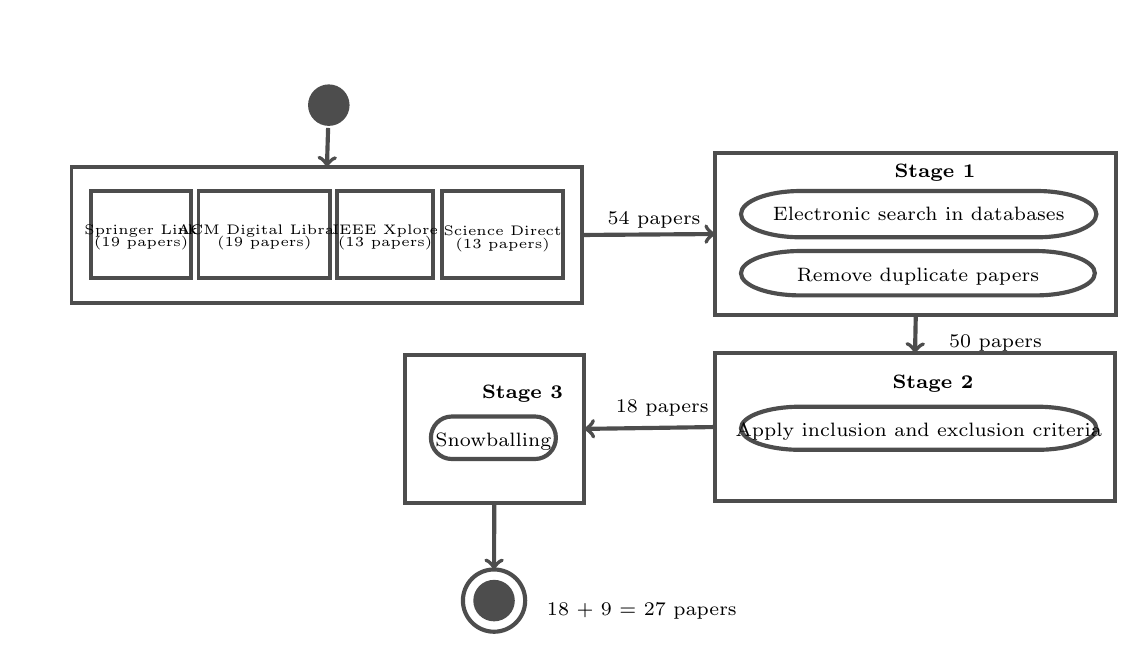
\begin{tikzpicture}
\pgftransformxscale{1.000000}
\pgftransformyscale{-1.000000}
\definecolor{dialinecolor}{rgb}{0.000000, 0.000000, 0.000000}
\pgfsetstrokecolor{dialinecolor}
\definecolor{dialinecolor}{rgb}{1.000000, 1.000000, 1.000000}
\pgfsetfillcolor{dialinecolor}
\definecolor{dialinecolor}{rgb}{1.000000, 1.000000, 1.000000}
\pgfsetfillcolor{dialinecolor}
\fill (-31.917258\du,3.529206\du)--(-31.917258\du,6.807243\du)--(-19.614266\du,6.807243\du)--(-19.614266\du,3.529206\du)--cycle;
\pgfsetlinewidth{0.090000\du}
\pgfsetdash{}{0pt}
\pgfsetdash{}{0pt}
\pgfsetmiterjoin
\definecolor{dialinecolor}{rgb}{0.301961, 0.301961, 0.301961}
\pgfsetstrokecolor{dialinecolor}
\draw (-31.917258\du,3.529206\du)--(-31.917258\du,6.807243\du)--(-19.614266\du,6.807243\du)--(-19.614266\du,3.529206\du)--cycle;
% setfont left to latex
\definecolor{dialinecolor}{rgb}{0.000000, 0.000000, 0.000000}
\pgfsetstrokecolor{dialinecolor}
\node at (-25.765762\du,5.249336\du){};
\definecolor{dialinecolor}{rgb}{1.000000, 1.000000, 1.000000}
\pgfsetfillcolor{dialinecolor}
\fill (-31.448657\du,4.108500\du)--(-31.448657\du,6.196277\du)--(-29.033657\du,6.196277\du)--(-29.033657\du,4.108500\du)--cycle;
\pgfsetlinewidth{0.090000\du}
\pgfsetdash{}{0pt}
\pgfsetdash{}{0pt}
\pgfsetmiterjoin
\definecolor{dialinecolor}{rgb}{0.301961, 0.301961, 0.301961}
\pgfsetstrokecolor{dialinecolor}
\draw (-31.448657\du,4.108500\du)--(-31.448657\du,6.196277\du)--(-29.033657\du,6.196277\du)--(-29.033657\du,4.108500\du)--cycle;
% setfont left to latex
\definecolor{dialinecolor}{rgb}{0.000000, 0.000000, 0.000000}
\pgfsetstrokecolor{dialinecolor}
\node at (-30.241157\du,5.075166\du){\tiny Springer Link};
% setfont left to latex
\definecolor{dialinecolor}{rgb}{0.000000, 0.000000, 0.000000}
\pgfsetstrokecolor{dialinecolor}
\node at (-30.241157\du,5.357389\du){\tiny (19 papers)};
\definecolor{dialinecolor}{rgb}{1.000000, 1.000000, 1.000000}
\pgfsetfillcolor{dialinecolor}
\fill (-28.859928\du,4.108500\du)--(-28.859928\du,6.196277\du)--(-25.689668\du,6.196277\du)--(-25.689668\du,4.108500\du)--cycle;
\pgfsetlinewidth{0.090000\du}
\pgfsetdash{}{0pt}
\pgfsetdash{}{0pt}
\pgfsetmiterjoin
\definecolor{dialinecolor}{rgb}{0.301961, 0.301961, 0.301961}
\pgfsetstrokecolor{dialinecolor}
\draw (-28.859928\du,4.108500\du)--(-28.859928\du,6.196277\du)--(-25.689668\du,6.196277\du)--(-25.689668\du,4.108500\du)--cycle;
% setfont left to latex
\definecolor{dialinecolor}{rgb}{0.000000, 0.000000, 0.000000}
\pgfsetstrokecolor{dialinecolor}
\node at (-27.274798\du,5.075166\du){\tiny ACM Digital Library};
% setfont left to latex
\definecolor{dialinecolor}{rgb}{0.000000, 0.000000, 0.000000}
\pgfsetstrokecolor{dialinecolor}
\node at (-27.274798\du,5.357389\du){\tiny (19 papers)};
% setfont left to latex
\definecolor{dialinecolor}{rgb}{0.000000, 0.000000, 0.000000}
\pgfsetstrokecolor{dialinecolor}
\node[anchor=west] at (-27.274798\du,5.152389\du){};
\definecolor{dialinecolor}{rgb}{1.000000, 1.000000, 1.000000}
\pgfsetfillcolor{dialinecolor}
\fill (-25.520498\du,4.108500\du)--(-25.520498\du,6.196277\du)--(-23.205498\du,6.196277\du)--(-23.205498\du,4.108500\du)--cycle;
\pgfsetlinewidth{0.090000\du}
\pgfsetdash{}{0pt}
\pgfsetdash{}{0pt}
\pgfsetmiterjoin
\definecolor{dialinecolor}{rgb}{0.301961, 0.301961, 0.301961}
\pgfsetstrokecolor{dialinecolor}
\draw (-25.520498\du,4.108500\du)--(-25.520498\du,6.196277\du)--(-23.205498\du,6.196277\du)--(-23.205498\du,4.108500\du)--cycle;
% setfont left to latex
\definecolor{dialinecolor}{rgb}{0.000000, 0.000000, 0.000000}
\pgfsetstrokecolor{dialinecolor}
\node at (-24.362998\du,5.075166\du){\tiny IEEE Xplore};
% setfont left to latex
\definecolor{dialinecolor}{rgb}{0.000000, 0.000000, 0.000000}
\pgfsetstrokecolor{dialinecolor}
\node at (-24.362998\du,5.357389\du){\tiny (13 papers)};
\definecolor{dialinecolor}{rgb}{1.000000, 1.000000, 1.000000}
\pgfsetfillcolor{dialinecolor}
\fill (-22.986880\du,4.108500\du)--(-22.986880\du,6.196277\du)--(-20.079380\du,6.196277\du)--(-20.079380\du,4.108500\du)--cycle;
\pgfsetlinewidth{0.090000\du}
\pgfsetdash{}{0pt}
\pgfsetdash{}{0pt}
\pgfsetmiterjoin
\definecolor{dialinecolor}{rgb}{0.301961, 0.301961, 0.301961}
\pgfsetstrokecolor{dialinecolor}
\draw (-22.986880\du,4.108500\du)--(-22.986880\du,6.196277\du)--(-20.079380\du,6.196277\du)--(-20.079380\du,4.108500\du)--cycle;
% setfont left to latex
\definecolor{dialinecolor}{rgb}{0.000000, 0.000000, 0.000000}
\pgfsetstrokecolor{dialinecolor}
\node at (-21.533130\du,5.057111\du){\tiny Science Direct};
% setfont left to latex
\definecolor{dialinecolor}{rgb}{0.000000, 0.000000, 0.000000}
\pgfsetstrokecolor{dialinecolor}
\node at (-21.533130\du,5.409889\du){\tiny (13 papers)};
\definecolor{dialinecolor}{rgb}{1.000000, 1.000000, 1.000000}
\pgfsetfillcolor{dialinecolor}
\fill (-16.409595\du,3.197689\du)--(-16.409595\du,7.093022\du)--(-6.750481\du,7.093022\du)--(-6.750481\du,3.197689\du)--cycle;
\pgfsetlinewidth{0.090000\du}
\pgfsetdash{}{0pt}
\pgfsetdash{}{0pt}
\pgfsetmiterjoin
\definecolor{dialinecolor}{rgb}{0.301961, 0.301961, 0.301961}
\pgfsetstrokecolor{dialinecolor}
\draw (-16.409595\du,3.197689\du)--(-16.409595\du,7.093022\du)--(-6.750481\du,7.093022\du)--(-6.750481\du,3.197689\du)--cycle;
% setfont left to latex
\definecolor{dialinecolor}{rgb}{0.000000, 0.000000, 0.000000}
\pgfsetstrokecolor{dialinecolor}
\node at (-11.580038\du,4.168133\du){};
% setfont left to latex
\definecolor{dialinecolor}{rgb}{0.000000, 0.000000, 0.000000}
\pgfsetstrokecolor{dialinecolor}
\node at (-11.580038\du,4.520911\du){};
% setfont left to latex
\definecolor{dialinecolor}{rgb}{0.000000, 0.000000, 0.000000}
\pgfsetstrokecolor{dialinecolor}
\node at (-11.580038\du,4.873689\du){};
% setfont left to latex
\definecolor{dialinecolor}{rgb}{0.000000, 0.000000, 0.000000}
\pgfsetstrokecolor{dialinecolor}
\node at (-11.580038\du,5.226466\du){};
% setfont left to latex
\definecolor{dialinecolor}{rgb}{0.000000, 0.000000, 0.000000}
\pgfsetstrokecolor{dialinecolor}
\node at (-11.580038\du,5.579244\du){};
% setfont left to latex
\definecolor{dialinecolor}{rgb}{0.000000, 0.000000, 0.000000}
\pgfsetstrokecolor{dialinecolor}
\node at (-11.580038\du,5.932022\du){};
% setfont left to latex
\definecolor{dialinecolor}{rgb}{0.000000, 0.000000, 0.000000}
\pgfsetstrokecolor{dialinecolor}
\node at (-11.580038\du,6.284800\du){};
% setfont left to latex
\definecolor{dialinecolor}{rgb}{0.000000, 0.000000, 0.000000}
\pgfsetstrokecolor{dialinecolor}
\node[anchor=west] at (-14.727183\du,10.833293\du){};
% setfont left to latex
\definecolor{dialinecolor}{rgb}{0.000000, 0.000000, 0.000000}
\pgfsetstrokecolor{dialinecolor}
\node[anchor=west] at (-11.580038\du,5.145355\du){};
\definecolor{dialinecolor}{rgb}{1.000000, 1.000000, 1.000000}
\pgfsetfillcolor{dialinecolor}
\fill (-16.409595\du,8.014929\du)--(-16.409595\du,11.574374\du)--(-6.787316\du,11.574374\du)--(-6.787316\du,8.014929\du)--cycle;
\pgfsetlinewidth{0.090000\du}
\pgfsetdash{}{0pt}
\pgfsetdash{}{0pt}
\pgfsetmiterjoin
\definecolor{dialinecolor}{rgb}{0.301961, 0.301961, 0.301961}
\pgfsetstrokecolor{dialinecolor}
\draw (-16.409595\du,8.014929\du)--(-16.409595\du,11.574374\du)--(-6.787316\du,11.574374\du)--(-6.787316\du,8.014929\du)--cycle;
% setfont left to latex
\definecolor{dialinecolor}{rgb}{0.000000, 0.000000, 0.000000}
\pgfsetstrokecolor{dialinecolor}
\node at (-11.598455\du,8.817429\du){};
% setfont left to latex
\definecolor{dialinecolor}{rgb}{0.000000, 0.000000, 0.000000}
\pgfsetstrokecolor{dialinecolor}
\node at (-11.598455\du,9.170207\du){};
% setfont left to latex
\definecolor{dialinecolor}{rgb}{0.000000, 0.000000, 0.000000}
\pgfsetstrokecolor{dialinecolor}
\node at (-11.598455\du,9.522985\du){};
% setfont left to latex
\definecolor{dialinecolor}{rgb}{0.000000, 0.000000, 0.000000}
\pgfsetstrokecolor{dialinecolor}
\node at (-11.598455\du,9.875763\du){};
% setfont left to latex
\definecolor{dialinecolor}{rgb}{0.000000, 0.000000, 0.000000}
\pgfsetstrokecolor{dialinecolor}
\node at (-11.598455\du,10.228540\du){};
% setfont left to latex
\definecolor{dialinecolor}{rgb}{0.000000, 0.000000, 0.000000}
\pgfsetstrokecolor{dialinecolor}
\node at (-11.598455\du,10.581318\du){};
% setfont left to latex
\definecolor{dialinecolor}{rgb}{0.000000, 0.000000, 0.000000}
\pgfsetstrokecolor{dialinecolor}
\node at (-11.598455\du,10.934096\du){};
% setfont left to latex
\definecolor{dialinecolor}{rgb}{0.000000, 0.000000, 0.000000}
\pgfsetstrokecolor{dialinecolor}
\node[anchor=west] at (-11.598455\du,9.794652\du){};
% setfont left to latex
\definecolor{dialinecolor}{rgb}{0.000000, 0.000000, 0.000000}
\pgfsetstrokecolor{dialinecolor}
\node[anchor=west] at (-12.122732\du,8.459829\du){};
% setfont left to latex
\definecolor{dialinecolor}{rgb}{0.000000, 0.000000, 0.000000}
\pgfsetstrokecolor{dialinecolor}
\node[anchor=west] at (-15.897732\du,9.584829\du){};
% setfont left to latex
\definecolor{dialinecolor}{rgb}{0.000000, 0.000000, 0.000000}
\pgfsetstrokecolor{dialinecolor}
\node[anchor=west] at (-12.154697\du,8.372549\du){};
% setfont left to latex
\definecolor{dialinecolor}{rgb}{0.000000, 0.000000, 0.000000}
\pgfsetstrokecolor{dialinecolor}
\node[anchor=west] at (-11.598455\du,9.794652\du){};
% setfont left to latex
\definecolor{dialinecolor}{rgb}{0.000000, 0.000000, 0.000000}
\pgfsetstrokecolor{dialinecolor}
\node[anchor=west] at (-12.974637\du,7.860073\du){};
% setfont left to latex
\definecolor{dialinecolor}{rgb}{0.000000, 0.000000, 0.000000}
\pgfsetstrokecolor{dialinecolor}
\node[anchor=west] at (-14.979697\du,8.522549\du){};
% setfont left to latex
\definecolor{dialinecolor}{rgb}{0.000000, 0.000000, 0.000000}
\pgfsetstrokecolor{dialinecolor}
\node[anchor=west] at (-10.466532\du,8.591129\du){};
\definecolor{dialinecolor}{rgb}{1.000000, 1.000000, 1.000000}
\pgfsetfillcolor{dialinecolor}
\fill (-23.887162\du,8.059949\du)--(-23.887162\du,11.619393\du)--(-19.569166\du,11.619393\du)--(-19.569166\du,8.059949\du)--cycle;
\pgfsetlinewidth{0.090000\du}
\pgfsetdash{}{0pt}
\pgfsetdash{}{0pt}
\pgfsetmiterjoin
\definecolor{dialinecolor}{rgb}{0.301961, 0.301961, 0.301961}
\pgfsetstrokecolor{dialinecolor}
\draw (-23.887162\du,8.059949\du)--(-23.887162\du,11.619393\du)--(-19.569166\du,11.619393\du)--(-19.569166\du,8.059949\du)--cycle;
% setfont left to latex
\definecolor{dialinecolor}{rgb}{0.000000, 0.000000, 0.000000}
\pgfsetstrokecolor{dialinecolor}
\node at (-21.728164\du,8.862449\du){};
% setfont left to latex
\definecolor{dialinecolor}{rgb}{0.000000, 0.000000, 0.000000}
\pgfsetstrokecolor{dialinecolor}
\node at (-21.728164\du,9.215226\du){};
% setfont left to latex
\definecolor{dialinecolor}{rgb}{0.000000, 0.000000, 0.000000}
\pgfsetstrokecolor{dialinecolor}
\node at (-21.728164\du,9.568004\du){};
% setfont left to latex
\definecolor{dialinecolor}{rgb}{0.000000, 0.000000, 0.000000}
\pgfsetstrokecolor{dialinecolor}
\node at (-21.728164\du,9.920782\du){};
% setfont left to latex
\definecolor{dialinecolor}{rgb}{0.000000, 0.000000, 0.000000}
\pgfsetstrokecolor{dialinecolor}
\node at (-21.728164\du,10.273560\du){};
% setfont left to latex
\definecolor{dialinecolor}{rgb}{0.000000, 0.000000, 0.000000}
\pgfsetstrokecolor{dialinecolor}
\node at (-21.728164\du,10.626338\du){};
% setfont left to latex
\definecolor{dialinecolor}{rgb}{0.000000, 0.000000, 0.000000}
\pgfsetstrokecolor{dialinecolor}
\node at (-21.728164\du,10.979115\du){};
% setfont left to latex
\definecolor{dialinecolor}{rgb}{0.000000, 0.000000, 0.000000}
\pgfsetstrokecolor{dialinecolor}
\node[anchor=west] at (-21.728164\du,9.839671\du){};
% setfont left to latex
\definecolor{dialinecolor}{rgb}{0.000000, 0.000000, 0.000000}
\pgfsetstrokecolor{dialinecolor}
\node[anchor=west] at (-22.296676\du,9.004456\du){\scriptsize \textbf{Stage 3}};
% setfont left to latex
\definecolor{dialinecolor}{rgb}{0.000000, 0.000000, 0.000000}
\pgfsetstrokecolor{dialinecolor}
\node[anchor=west] at (-17.469006\du,11.002467\du){};
% setfont left to latex
\definecolor{dialinecolor}{rgb}{0.000000, 0.000000, 0.000000}
\pgfsetstrokecolor{dialinecolor}
\node[anchor=west] at (-22.385901\du,10.417810\du){};
% setfont left to latex
\definecolor{dialinecolor}{rgb}{0.000000, 0.000000, 0.000000}
\pgfsetstrokecolor{dialinecolor}
\node[anchor=west] at (-21.728164\du,9.839671\du){};
% setfont left to latex
\definecolor{dialinecolor}{rgb}{0.000000, 0.000000, 0.000000}
\pgfsetstrokecolor{dialinecolor}
\node[anchor=west] at (-30.104804\du,11.393752\du){};
% setfont left to latex
\definecolor{dialinecolor}{rgb}{0.000000, 0.000000, 0.000000}
\pgfsetstrokecolor{dialinecolor}
\node[anchor=west] at (-26.271407\du,8.805627\du){};
% setfont left to latex
\definecolor{dialinecolor}{rgb}{0.000000, 0.000000, 0.000000}
\pgfsetstrokecolor{dialinecolor}
\node[anchor=west] at (-21.985901\du,10.425310\du){};
\pgfsetlinewidth{0.100000\du}
\pgfsetdash{}{0pt}
\pgfsetdash{}{0pt}
\pgfsetbuttcap
\pgfsetmiterjoin
\pgfsetlinewidth{0.100000\du}
\pgfsetbuttcap
\pgfsetmiterjoin
\pgfsetdash{}{0pt}
\definecolor{dialinecolor}{rgb}{1.000000, 1.000000, 1.000000}
\pgfsetfillcolor{dialinecolor}
\pgfpathmoveto{\pgfpoint{-14.364235\du}{4.109362\du}}
\pgfpathlineto{\pgfpoint{-8.656319\du}{4.109362\du}}
\pgfpathcurveto{\pgfpoint{-7.868219\du}{4.109362\du}}{\pgfpoint{-7.229340\du}{4.358800\du}}{\pgfpoint{-7.229340\du}{4.666496\du}}
\pgfpathcurveto{\pgfpoint{-7.229340\du}{4.974193\du}}{\pgfpoint{-7.868219\du}{5.223630\du}}{\pgfpoint{-8.656319\du}{5.223630\du}}
\pgfpathlineto{\pgfpoint{-14.364235\du}{5.223630\du}}
\pgfpathcurveto{\pgfpoint{-15.152334\du}{5.223630\du}}{\pgfpoint{-15.791214\du}{4.974193\du}}{\pgfpoint{-15.791214\du}{4.666496\du}}
\pgfpathcurveto{\pgfpoint{-15.791214\du}{4.358800\du}}{\pgfpoint{-15.152334\du}{4.109362\du}}{\pgfpoint{-14.364235\du}{4.109362\du}}
\pgfusepath{fill}
\definecolor{dialinecolor}{rgb}{0.301961, 0.301961, 0.301961}
\pgfsetstrokecolor{dialinecolor}
\pgfpathmoveto{\pgfpoint{-14.364235\du}{4.109362\du}}
\pgfpathlineto{\pgfpoint{-8.656319\du}{4.109362\du}}
\pgfpathcurveto{\pgfpoint{-7.868219\du}{4.109362\du}}{\pgfpoint{-7.229340\du}{4.358800\du}}{\pgfpoint{-7.229340\du}{4.666496\du}}
\pgfpathcurveto{\pgfpoint{-7.229340\du}{4.974193\du}}{\pgfpoint{-7.868219\du}{5.223630\du}}{\pgfpoint{-8.656319\du}{5.223630\du}}
\pgfpathlineto{\pgfpoint{-14.364235\du}{5.223630\du}}
\pgfpathcurveto{\pgfpoint{-15.152334\du}{5.223630\du}}{\pgfpoint{-15.791214\du}{4.974193\du}}{\pgfpoint{-15.791214\du}{4.666496\du}}
\pgfpathcurveto{\pgfpoint{-15.791214\du}{4.358800\du}}{\pgfpoint{-15.152334\du}{4.109362\du}}{\pgfpoint{-14.364235\du}{4.109362\du}}
\pgfusepath{stroke}
% setfont left to latex
\definecolor{dialinecolor}{rgb}{0.000000, 0.000000, 0.000000}
\pgfsetstrokecolor{dialinecolor}
\node at (-11.510277\du,4.654691\du){\scriptsize Electronic search in databases};
% setfont left to latex
\definecolor{dialinecolor}{rgb}{0.000000, 0.000000, 0.000000}
\pgfsetstrokecolor{dialinecolor}
\node[anchor=west] at (-11.510277\du,4.666496\du){};
% setfont left to latex
\definecolor{dialinecolor}{rgb}{0.000000, 0.000000, 0.000000}
\pgfsetstrokecolor{dialinecolor}
\node[anchor=west] at (-11.580038\du,5.145355\du){};
\pgfsetlinewidth{0.100000\du}
\pgfsetdash{}{0pt}
\pgfsetdash{}{0pt}
\pgfsetbuttcap
\pgfsetmiterjoin
\pgfsetlinewidth{0.100000\du}
\pgfsetbuttcap
\pgfsetmiterjoin
\pgfsetdash{}{0pt}
\definecolor{dialinecolor}{rgb}{1.000000, 1.000000, 1.000000}
\pgfsetfillcolor{dialinecolor}
\pgfpathmoveto{\pgfpoint{-14.370374\du}{5.555148\du}}
\pgfpathlineto{\pgfpoint{-8.687015\du}{5.555148\du}}
\pgfpathcurveto{\pgfpoint{-7.902306\du}{5.555148\du}}{\pgfpoint{-7.266175\du}{5.794278\du}}{\pgfpoint{-7.266175\du}{6.089260\du}}
\pgfpathcurveto{\pgfpoint{-7.266175\du}{6.384242\du}}{\pgfpoint{-7.902306\du}{6.623372\du}}{\pgfpoint{-8.687015\du}{6.623372\du}}
\pgfpathlineto{\pgfpoint{-14.370374\du}{6.623372\du}}
\pgfpathcurveto{\pgfpoint{-15.155083\du}{6.623372\du}}{\pgfpoint{-15.791214\du}{6.384242\du}}{\pgfpoint{-15.791214\du}{6.089260\du}}
\pgfpathcurveto{\pgfpoint{-15.791214\du}{5.794278\du}}{\pgfpoint{-15.155083\du}{5.555148\du}}{\pgfpoint{-14.370374\du}{5.555148\du}}
\pgfusepath{fill}
\definecolor{dialinecolor}{rgb}{0.301961, 0.301961, 0.301961}
\pgfsetstrokecolor{dialinecolor}
\pgfpathmoveto{\pgfpoint{-14.370374\du}{5.555148\du}}
\pgfpathlineto{\pgfpoint{-8.687015\du}{5.555148\du}}
\pgfpathcurveto{\pgfpoint{-7.902306\du}{5.555148\du}}{\pgfpoint{-7.266175\du}{5.794278\du}}{\pgfpoint{-7.266175\du}{6.089260\du}}
\pgfpathcurveto{\pgfpoint{-7.266175\du}{6.384242\du}}{\pgfpoint{-7.902306\du}{6.623372\du}}{\pgfpoint{-8.687015\du}{6.623372\du}}
\pgfpathlineto{\pgfpoint{-14.370374\du}{6.623372\du}}
\pgfpathcurveto{\pgfpoint{-15.155083\du}{6.623372\du}}{\pgfpoint{-15.791214\du}{6.384242\du}}{\pgfpoint{-15.791214\du}{6.089260\du}}
\pgfpathcurveto{\pgfpoint{-15.791214\du}{5.794278\du}}{\pgfpoint{-15.155083\du}{5.555148\du}}{\pgfpoint{-14.370374\du}{5.555148\du}}
\pgfusepath{stroke}
% setfont left to latex
\definecolor{dialinecolor}{rgb}{0.000000, 0.000000, 0.000000}
\pgfsetstrokecolor{dialinecolor}
\node at (-11.528694\du,6.177454\du){\scriptsize Remove duplicate papers};
% setfont left to latex
\definecolor{dialinecolor}{rgb}{0.000000, 0.000000, 0.000000}
\pgfsetstrokecolor{dialinecolor}
\node[anchor=west] at (-11.510277\du,4.666496\du){};
\pgfsetlinewidth{0.100000\du}
\pgfsetdash{}{0pt}
\pgfsetdash{}{0pt}
\pgfsetbuttcap
\pgfsetmiterjoin
\pgfsetlinewidth{0.100000\du}
\pgfsetbuttcap
\pgfsetmiterjoin
\pgfsetdash{}{0pt}
\definecolor{dialinecolor}{rgb}{1.000000, 1.000000, 1.000000}
\pgfsetfillcolor{dialinecolor}
\pgfpathmoveto{\pgfpoint{-14.364235\du}{9.305335\du}}
\pgfpathlineto{\pgfpoint{-8.656319\du}{9.305335\du}}
\pgfpathcurveto{\pgfpoint{-7.868219\du}{9.305335\du}}{\pgfpoint{-7.229340\du}{9.537789\du}}{\pgfpoint{-7.229340\du}{9.824536\du}}
\pgfpathcurveto{\pgfpoint{-7.229340\du}{10.111283\du}}{\pgfpoint{-7.868219\du}{10.343738\du}}{\pgfpoint{-8.656319\du}{10.343738\du}}
\pgfpathlineto{\pgfpoint{-14.364235\du}{10.343738\du}}
\pgfpathcurveto{\pgfpoint{-15.152334\du}{10.343738\du}}{\pgfpoint{-15.791214\du}{10.111283\du}}{\pgfpoint{-15.791214\du}{9.824536\du}}
\pgfpathcurveto{\pgfpoint{-15.791214\du}{9.537789\du}}{\pgfpoint{-15.152334\du}{9.305335\du}}{\pgfpoint{-14.364235\du}{9.305335\du}}
\pgfusepath{fill}
\definecolor{dialinecolor}{rgb}{0.301961, 0.301961, 0.301961}
\pgfsetstrokecolor{dialinecolor}
\pgfpathmoveto{\pgfpoint{-14.364235\du}{9.305335\du}}
\pgfpathlineto{\pgfpoint{-8.656319\du}{9.305335\du}}
\pgfpathcurveto{\pgfpoint{-7.868219\du}{9.305335\du}}{\pgfpoint{-7.229340\du}{9.537789\du}}{\pgfpoint{-7.229340\du}{9.824536\du}}
\pgfpathcurveto{\pgfpoint{-7.229340\du}{10.111283\du}}{\pgfpoint{-7.868219\du}{10.343738\du}}{\pgfpoint{-8.656319\du}{10.343738\du}}
\pgfpathlineto{\pgfpoint{-14.364235\du}{10.343738\du}}
\pgfpathcurveto{\pgfpoint{-15.152334\du}{10.343738\du}}{\pgfpoint{-15.791214\du}{10.111283\du}}{\pgfpoint{-15.791214\du}{9.824536\du}}
\pgfpathcurveto{\pgfpoint{-15.791214\du}{9.537789\du}}{\pgfpoint{-15.152334\du}{9.305335\du}}{\pgfpoint{-14.364235\du}{9.305335\du}}
\pgfusepath{stroke}
% setfont left to latex
\definecolor{dialinecolor}{rgb}{0.000000, 0.000000, 0.000000}
\pgfsetstrokecolor{dialinecolor}
\node at (-11.510277\du,9.912731\du){\scriptsize Apply inclusion and exclusion criteria};
\pgfsetlinewidth{0.100000\du}
\pgfsetdash{}{0pt}
\pgfsetdash{}{0pt}
\pgfsetbuttcap
\pgfsetmiterjoin
\pgfsetlinewidth{0.100000\du}
\pgfsetbuttcap
\pgfsetmiterjoin
\pgfsetdash{}{0pt}
\definecolor{dialinecolor}{rgb}{1.000000, 1.000000, 1.000000}
\pgfsetfillcolor{dialinecolor}
\pgfpathmoveto{\pgfpoint{-22.759086\du}{9.541292\du}}
\pgfpathlineto{\pgfpoint{-20.751586\du}{9.541292\du}}
\pgfpathcurveto{\pgfpoint{-20.474408\du}{9.541292\du}}{\pgfpoint{-20.249711\du}{9.770400\du}}{\pgfpoint{-20.249711\du}{10.053021\du}}
\pgfpathcurveto{\pgfpoint{-20.249711\du}{10.335641\du}}{\pgfpoint{-20.474408\du}{10.564749\du}}{\pgfpoint{-20.751586\du}{10.564749\du}}
\pgfpathlineto{\pgfpoint{-22.759086\du}{10.564749\du}}
\pgfpathcurveto{\pgfpoint{-23.036264\du}{10.564749\du}}{\pgfpoint{-23.260961\du}{10.335641\du}}{\pgfpoint{-23.260961\du}{10.053021\du}}
\pgfpathcurveto{\pgfpoint{-23.260961\du}{9.770400\du}}{\pgfpoint{-23.036264\du}{9.541292\du}}{\pgfpoint{-22.759086\du}{9.541292\du}}
\pgfusepath{fill}
\definecolor{dialinecolor}{rgb}{0.301961, 0.301961, 0.301961}
\pgfsetstrokecolor{dialinecolor}
\pgfpathmoveto{\pgfpoint{-22.759086\du}{9.541292\du}}
\pgfpathlineto{\pgfpoint{-20.751586\du}{9.541292\du}}
\pgfpathcurveto{\pgfpoint{-20.474408\du}{9.541292\du}}{\pgfpoint{-20.249711\du}{9.770400\du}}{\pgfpoint{-20.249711\du}{10.053021\du}}
\pgfpathcurveto{\pgfpoint{-20.249711\du}{10.335641\du}}{\pgfpoint{-20.474408\du}{10.564749\du}}{\pgfpoint{-20.751586\du}{10.564749\du}}
\pgfpathlineto{\pgfpoint{-22.759086\du}{10.564749\du}}
\pgfpathcurveto{\pgfpoint{-23.036264\du}{10.564749\du}}{\pgfpoint{-23.260961\du}{10.335641\du}}{\pgfpoint{-23.260961\du}{10.053021\du}}
\pgfpathcurveto{\pgfpoint{-23.260961\du}{9.770400\du}}{\pgfpoint{-23.036264\du}{9.541292\du}}{\pgfpoint{-22.759086\du}{9.541292\du}}
\pgfusepath{stroke}
% setfont left to latex
\definecolor{dialinecolor}{rgb}{0.000000, 0.000000, 0.000000}
\pgfsetstrokecolor{dialinecolor}
\node at (-21.755336\du,10.141215\du){\scriptsize Snowballing};
\pgfsetlinewidth{0.100000\du}
\pgfsetdash{}{0pt}
\pgfsetdash{}{0pt}
\pgfsetbuttcap
{
\definecolor{dialinecolor}{rgb}{0.301961, 0.301961, 0.301961}
\pgfsetfillcolor{dialinecolor}
% was here!!!
\pgfsetarrowsend{to}
\definecolor{dialinecolor}{rgb}{0.301961, 0.301961, 0.301961}
\pgfsetstrokecolor{dialinecolor}
\draw (-19.614266\du,5.168224\du)--(-16.409595\du,5.145355\du);
}
\pgfsetlinewidth{0.100000\du}
\pgfsetdash{}{0pt}
\pgfsetdash{}{0pt}
\pgfsetbuttcap
{
\definecolor{dialinecolor}{rgb}{0.301961, 0.301961, 0.301961}
\pgfsetfillcolor{dialinecolor}
% was here!!!
\pgfsetarrowsend{to}
\definecolor{dialinecolor}{rgb}{0.301961, 0.301961, 0.301961}
\pgfsetstrokecolor{dialinecolor}
\draw (-11.580038\du,7.093022\du)--(-11.598455\du,8.014929\du);
}
\pgfsetlinewidth{0.100000\du}
\pgfsetdash{}{0pt}
\pgfsetdash{}{0pt}
\pgfsetbuttcap
{
\definecolor{dialinecolor}{rgb}{0.301961, 0.301961, 0.301961}
\pgfsetfillcolor{dialinecolor}
% was here!!!
\pgfsetarrowsend{to}
\definecolor{dialinecolor}{rgb}{0.301961, 0.301961, 0.301961}
\pgfsetstrokecolor{dialinecolor}
\draw (-16.409595\du,9.794652\du)--(-19.569166\du,9.839671\du);
}
% setfont left to latex
\definecolor{dialinecolor}{rgb}{0.301961, 0.301961, 0.301961}
\pgfsetstrokecolor{dialinecolor}
\node[anchor=west] at (-19.275615\du,4.813556\du){\scriptsize 54 papers};
% setfont left to latex
\definecolor{dialinecolor}{rgb}{0.301961, 0.301961, 0.301961}
\pgfsetstrokecolor{dialinecolor}
\node[anchor=west] at (-11.052270\du,7.784965\du){\scriptsize 50 papers};
% setfont left to latex
\definecolor{dialinecolor}{rgb}{0.000000, 0.000000, 0.000000}
\pgfsetstrokecolor{dialinecolor}
\node[anchor=west] at (-21.429176\du,7.178609\du){};
% setfont left to latex
\definecolor{dialinecolor}{rgb}{0.301961, 0.301961, 0.301961}
\pgfsetstrokecolor{dialinecolor}
\node[anchor=west] at (-19.080362\du,9.338528\du){\scriptsize 18 papers};
\pgfsetlinewidth{0.100000\du}
\pgfsetdash{}{0pt}
\definecolor{dialinecolor}{rgb}{1.000000, 1.000000, 1.000000}
\pgfsetfillcolor{dialinecolor}
\pgfpathellipse{\pgfpoint{-21.739730\du}{13.975896\du}}{\pgfpoint{0.750000\du}{0\du}}{\pgfpoint{0\du}{0.750000\du}}
\pgfusepath{fill}
\definecolor{dialinecolor}{rgb}{0.301961, 0.301961, 0.301961}
\pgfsetstrokecolor{dialinecolor}
\pgfpathellipse{\pgfpoint{-21.739730\du}{13.975896\du}}{\pgfpoint{0.750000\du}{0\du}}{\pgfpoint{0\du}{0.750000\du}}
\pgfusepath{stroke}
\definecolor{dialinecolor}{rgb}{0.301961, 0.301961, 0.301961}
\pgfsetfillcolor{dialinecolor}
\pgfpathellipse{\pgfpoint{-21.739730\du}{13.975896\du}}{\pgfpoint{0.500000\du}{0\du}}{\pgfpoint{0\du}{0.500000\du}}
\pgfusepath{fill}
\pgfsetlinewidth{0.100000\du}
\pgfsetdash{}{0pt}
\pgfsetdash{}{0pt}
\pgfsetbuttcap
{
\definecolor{dialinecolor}{rgb}{0.301961, 0.301961, 0.301961}
\pgfsetfillcolor{dialinecolor}
% was here!!!
\pgfsetarrowsend{to}
\definecolor{dialinecolor}{rgb}{0.301961, 0.301961, 0.301961}
\pgfsetstrokecolor{dialinecolor}
\draw (-21.734353\du,11.651831\du)--(-21.739730\du,13.225896\du);
}
\pgfsetlinewidth{0.100000\du}
\pgfsetdash{}{0pt}
\definecolor{dialinecolor}{rgb}{0.301961, 0.301961, 0.301961}
\pgfsetfillcolor{dialinecolor}
\pgfpathellipse{\pgfpoint{-25.720406\du}{2.040372\du}}{\pgfpoint{0.500000\du}{0\du}}{\pgfpoint{0\du}{0.500000\du}}
\pgfusepath{fill}
\pgfsetlinewidth{0.100000\du}
\pgfsetdash{}{0pt}
\pgfsetdash{}{0pt}
\pgfsetbuttcap
{
\definecolor{dialinecolor}{rgb}{0.301961, 0.301961, 0.301961}
\pgfsetfillcolor{dialinecolor}
% was here!!!
\pgfsetarrowsend{to}
\definecolor{dialinecolor}{rgb}{0.301961, 0.301961, 0.301961}
\pgfsetstrokecolor{dialinecolor}
\draw (-25.737160\du,2.590325\du)--(-25.765762\du,3.529206\du);
}
% setfont left to latex
\definecolor{dialinecolor}{rgb}{0.000000, 0.000000, 0.000000}
\pgfsetstrokecolor{dialinecolor}
\node[anchor=west] at (-10.434011\du,3.418700\du){};
% setfont left to latex
\definecolor{dialinecolor}{rgb}{0.301961, 0.301961, 0.301961}
\pgfsetstrokecolor{dialinecolor}
\node[anchor=west] at (-20.736845\du,14.238237\du){\scriptsize 18 + 9 = 27 papers};
% setfont left to latex
\definecolor{dialinecolor}{rgb}{0.301961, 0.301961, 0.301961}
\pgfsetstrokecolor{dialinecolor}
\node[anchor=west] at (-31.713766\du,0.646010\du){};
% setfont left to latex
\definecolor{dialinecolor}{rgb}{0.000000, 0.000000, 0.000000}
\pgfsetstrokecolor{dialinecolor}
\node[anchor=west] at (-12.364726\du,3.677517\du){\scriptsize \textbf{Stage 1}};
% setfont left to latex
\definecolor{dialinecolor}{rgb}{0.000000, 0.000000, 0.000000}
\pgfsetstrokecolor{dialinecolor}
\node[anchor=west] at (-11.723247\du,3.750218\du){};
% setfont left to latex
\definecolor{dialinecolor}{rgb}{0.000000, 0.000000, 0.000000}
\pgfsetstrokecolor{dialinecolor}
\node[anchor=west] at (-33.025103\du,0.396474\du){};
% setfont left to latex
\definecolor{dialinecolor}{rgb}{0.000000, 0.000000, 0.000000}
\pgfsetstrokecolor{dialinecolor}
\node[anchor=west] at (-33.025103\du,0.396474\du){};
% setfont left to latex
\definecolor{dialinecolor}{rgb}{0.000000, 0.000000, 0.000000}
\pgfsetstrokecolor{dialinecolor}
\node[anchor=west] at (-12.413156\du,8.757105\du){\scriptsize \textbf{Stage 2}};
\end{tikzpicture}

  \includegraphics[width=.9\textwidth]{figures/smr-selection-phases.pdf}
  \caption{Diagram of the four-stage paper selection process.}
  \label{fig:smr_selection_phases}
\end{figure}

\begin{table*}[h!]
  \centering
  \spacebtrows{1.3}
  \caption{Selected papers}
  \begin{tabular}{@{}lp{18cm}@{}} 
    \toprule
    ID & Bibliographic reference\\ 
    \midrule
    %  \#1 & A. Lamkanfi, S. Demeyer, E. Giger and B. Goethals, ``Predicting the severity of a reported bug," 2010 7th IEEE Working Conference on Mining Software Repositories (MSR 2010), Cape Town, 2010, pp. 1-10.\\
    \cite{Lamkanfi:2010} & \vspace{-0.2cm}\bibentry{Lamkanfi:2010}. doi:\href{https://doi.org/10.1109/MSR.2010.5463284}{10.1109/MSR.2010.5463284}.\\
    
    %  \#2 & A. Lamkanfi, S. Demeyer, Q. D. Soetens and T. Verdonck, ``Comparing Mining Algorithms for Predicting the Severity of a Reported Bug", 2011 15th European Conference on Software Maintenance and Reengineering, Oldenburg, 2011, pp. 249-258.\\
    \cite{Lamkanfi:2011} & \vspace{-0.2cm}\bibentry{Lamkanfi:2011}. doi:\href{https://doi.org/10.1109/CSMR.2011.31}{10.1109/CSMR.2011.31}.\\
    
    %  \#3 & Y. Tian, D. Lo and C. Sun, ``Information Retrieval Based Nearest Neighbor Classification for Fine-Grained Bug Severity Prediction," 2012 19th Working Conference on Reverse Engineering, Kingston, ON, 2012, pp. 215-224.\\ 
    \cite{Tian:2012} & \vspace{-0.2cm}\bibentry{Tian:2012}.  doi:\href{https://doi.org/10.1109/WCRE.2012.31}{10.1109/WCRE.2012.31}.\\
    
    %  \#4 & C. Z. Yang, C. C. Hou, W. C. Kao and I. X. Chen, ``An Empirical Study on Improving Severity Prediction of Defect Reports Using Feature Selection," 2012 19th Asia-Pacific Software Engineering Conference, Hong Kong, 2012, pp. 240-249.\\
    \cite{Yang:2012} & \vspace{-0.2cm}\bibentry{Yang:2012}.  doi:\href{https://doi.org/10.1109/APSEC.2012.144}{10.1109/APSEC.2012.144}.\\
    
    %  \#5 & Chaturvedi, K. K. and V.B. Singh. ``An Empirical Comparison of Machine Learning Techniques in Predicting the Bug Severity of Open and Closed Source Projects." IJOSSP 4.2 (2012): 32-59. \\ 
    \cite{Chaturvedi:2012} & \vspace{-0.2cm}\bibentry{Chaturvedi:2012}.  doi:\href{https://doi.org/10.4018/jossp.2012040103}{10.4018/jossp.2012040103}.\\
    
    %  \#6 & C. Z. Yang, K. Y. Chen, W. C. Kao and C. C. Yang, ``Improving severity prediction on software bug reports using quality indicators," 2014 IEEE 5th International Conference on Software Engineering and Service Science, Beijing, 2014, pp. 216-219.\\ 
    \cite{Yang:2014a} & \vspace{-0.2cm}\bibentry{Yang:2014a}.  doi:\href{https://doi.org/10.1109/ICSESS.2014.6933548}{10.1109/ICSESS.2014.6933548}.\\ 
    
    %  \#7 & G. Yang, T. Zhang and B. Lee, ``Towards Semi-automatic Bug Triage and Severity Prediction Based on Topic Model and Multi-feature of Bug Reports," 2014 IEEE 38th Annual Computer Software and Applications Conference, Vasteras, 2014, pp. 97-106.\\ 
    \cite{Yang:2014b} & \vspace{-0.2cm}\bibentry{Yang:2014b}.  doi:\href{https://doi.org/10.1109/COMPSAC.2014.16}{10.1109/COMPSAC.2014.16}.\\
    
    %  \#8 & Harold Valdivia Garcia and Emad Shihab. 2014. ``Characterizing and predicting blocking bugs in open source projects". In Proceedings of the 11th Working Conference on Mining Software Repositories (MSR 2014). ACM, New York, NY, USA, 72-81.\\
    \cite{Valdivia:2014} & \vspace{-0.2cm}\bibentry{Valdivia:2014}.  doi:\href{https://doi.org/10.1145/2597073.2597099}{10.1145/2597073.2597099}\\
    
    %  \#9 & Sharma M., Kumari M., Singh R.K., Singh V.B. (2014) ``Multiattribute Based Machine Learning Models for Severity Prediction in Cross Project Context". In: Murgante B. et al. (eds) Computational Science and Its Applications – ICCSA 2014. ICCSA 2014. Lecture Notes in Computer Science, vol 8583. Springer, Cham.\\ 
    \cite{Meera:2014} & \vspace{-0.2cm}\bibentry{Meera:2014}.  doi:\href{https://doi.org/10.1007/978-3-319-09156-3\_17}{10.1007/978-3-319-09156-3\_17}\\
    
    %  \#10 & N. K. S. Roy and B. Rossi, ``Towards an Improvement of Bug Severity Classification," 2014 40th EUROMICRO Conference on Software Engineering and Advanced Applications, Verona, 2014, pp. 269-276.\\ 
    \cite{Roy:2014} & \vspace{-0.2cm}\bibentry{Roy:2014}.  doi:\href{https://doi.org/10.1109/SEAA.2014.51}{10.1109/SEAA.2014.51}\\
    
    %  \#11 & Ripon K. Saha, Julia Lawall, Sarfraz Khurshid, and Dewayne E. Perry. 2015. ``Are these bugs really ``normal"?''. In Proceedings of the 12th Working Conference on Mining Software Repositories (MSR '15). IEEE Press, Piscataway, NJ, USA, 258-268.\\ 
    \cite{Saha:2015} & \vspace{-0.2cm}\bibentry{Saha:2015}.  doi:\href{https://doi.org/10.1109/MSR.2015.31}{10.1109/MSR.2015.31}\\
    
    %  \#12 & Tao Zhang, Geunseok Yang, Byungjeong Lee, and Alvin T. S. Chan. 2015. ``Predicting severity of bug report by mining bug repository with concept profile". In Proceedings of the 30th Annual ACM Symposium on Applied Computing (SAC '15). ACM, New York, NY, USA, 1553-1558.\\ 
    \cite{Zhang:2015} & \vspace{-0.2cm}\bibentry{Zhang:2015}.  doi:\href{https://doi.org/10.1145/2695664.2695872}{10.1145/2695664.2695872}\\
    
    %  \#13 & G. Sharma, S. Sharma, S. Gujral, ``A Novel Way of Assessing Software Bug Severity Using Dictionary of Critical Terms", Procedia Computer Science, pp. 632-639, 2015.\\ 
    \cite{Sharma:2015} & \vspace{-0.2cm}\bibentry{Sharma:2015}.  doi:\href{https://doi.org/10.1016/j.procs.2015.10.059}{10.1016/j.procs.2015.10.059}\\
    
    %  \#14 & X. Xia, D. Lo, E. Shihab, X. Wang, X. Yang, ``Elblocker: Predicting blocking bugs with ensemble imbalance learning", Information and Software Technology, 2015.\\ 
    \cite{Xia:2015} & \vspace{-0.2cm}\bibentry{Xia:2015}.  doi:\href{https://doi.org/10.1016/j.infsof.2014.12.006}{10.1016/j.infsof.2014.12.006}\\
    
    %  \#15 & S. Gujral, G. Sharma, S. Sharma and Diksha, ``Classifying bug severity using dictionary-based approach," 2015 International Conference on Futuristic Trends on Computational Analysis and Knowledge Management (ABLAZE), Noida, 2015, pp. 599-602.\\ 
    \cite{Gujral:2015} & \vspace{-0.2cm}\bibentry{Gujral:2015}.  doi:\href{https://doi.org/10.1109/ABLAZE.2015.7154933}{10.1109/ABLAZE.2015.7154933}\\
    
    %  \#16 & M. N. Pushpalatha and M. Mrunalini, ``Predicting the severity of bug reports using classification algorithms," 2016 International Conference on Circuits, Controls, Communications and Computing (I4C), Bangalore, 2016, pp. 1-4.\\ 
    \cite{Pushpalathas:2016} & \vspace{-0.2cm}\bibentry{Pushpalathas:2016}.  doi:\href{https://doi.org/10.1109/CIMCA.2016.8053276}{10.1109/CIMCA.2016.8053276}\\
    
    %  \#17 & A. F. Otoom, D. Al-Shdaifat, M. Hammad and E. E. Abdallah, ``Severity prediction of software bugs," 2016 7th International Conference on Information and Communication Systems (ICICS), Irbid, 2016, pp. 92-95.\\ 
    \cite{Otoom:2016} & \vspace{-0.2cm}\bibentry{Otoom:2016}.  doi:\href{https://doi.org/10.1109/IACS.2016.7476092}{10.1109/IACS.2016.7476092}\\  
    
    % \#18 & Korosh Koochekian Sabor, Mohammad Hamdaqa, and Abdelwahab Hamou-Lhadj. 2016. ``Automatic prediction of the severity of bugs using stack traces". In Proceedings of the 26th Annual International Conference on Computer Science and Software Engineering (CASCON '16), Blake Jones (Ed.). IBM Corp., Riverton, NJ, USA, 96-105. \\ 
    \cite{Sabor:2016} & \vspace{-0.2cm}\bibentry{Sabor:2016}.\\  
    
    %  \#19 & Tian, Y., Ali, N., Lo, D. et al. Empir Software Eng (2016) 21: 2298. https://doi.org/10.1007/s10664-015-9409-1\\ 
    \cite{Tian:2016} & \vspace{-0.2cm}\bibentry{Tian:2016}.  doi:\href{https://doi.org/10.1007/s10664-015-9409-1}{10.1007/s10664-015-9409-1}\\
    
    %  \#20 & Tao Zhang, Jiachi Chen, Geunseok Yang, Byungjeong Lee, and Xiapu Luo. 2016. ``Towards more accurate severity prediction and fixer recommendation of software bugs". J. Syst. Softw. 117, C (July 2016), 166-184. \\ 
    \cite{Zhang:2016} & \vspace{-0.2cm}\bibentry{Zhang:2016}.  doi:\href{https://doi.org/10.1016/j.jss.2016.02.034}{10.1016/j.jss.2016.02.034}\\
    
    %  \#21 & Kwanghue, J., Amarmend, D., Geunseok, Y., Jung-Won, L., Byungjeong, L.: ``Bug severity prediction by classifying normal bugs with text and meta-field information". Adv. Sci. Technol. Lett. 129 (2016). Mechanical Engineering.\\ 
    \cite{Jin:2016a} & \vspace{-0.2cm}\bibentry{Jin:2016a}.  doi:\href{http://dx.doi.org/10.14257/astl.2016.129.05}{10.14257/astl.2016.129.05}\\
    
    %  \#22 & T. Choeikiwong, P. Vateekul, ``Improve accuracy of defect severity categorization using semi-supervised approach on imbalanced data sets", Proceedings of the International MultiConference of Engineers and Computer Scientists, vol. 1, 2016.\\ 
    \cite{Choeikiwong:2016} & \vspace{-0.2cm}\bibentry{Choeikiwong:2016}.\\
    
    %  \#23 & Jin, Kwanghue, Dashbalbar, Amarmend Yang, Geunseok, Lee, Byungjeong, Lee, Jung-Won. (2016). ``Improving predictions about bug severity by utilizing bugs classified as normal". Contemporary Engineering Sciences. 9. 933-942. 10.12988/ces.2016.6695.\\ 
    \cite{Jin:2016b} & \vspace{-0.2cm}\bibentry{Jin:2016b}.  doi:\href{http://dx.doi.org/10.12988/ces.2016.6695}{10.12988/ces.2016.6695}\\
    
    %  \#24 & Jin, K, Lee, E.C., Dashbalbar, A, Lee, J, Lee, B. (2016). ``Utilizing feature based classification and textual information of bug reports for severity prediction". 19. 651-659. \\
    \cite{Jin:2016c} & \vspace{-0.2cm}\bibentry{Jin:2016c}.\\
    
    %  \#25 & Geunseok Yang, Seungsuk Baek, Jung-Won Lee, and Byungjeong Lee. 2017. ``Analyzing emotion words to predict severity of software bugs: a case study of open source projects". In Proceedings of the Symposium on Applied Computing (SAC '17). ACM, New York, NY, USA, 1280-1287. \\ 
    \cite{Yang:2017} & \vspace{-0.2cm}\bibentry{Yang:2017}.  doi:\href{http://doi.org/10.1145/3019612.3019788}{10.1145/3019612.3019788}\\
    
    %  \#26 & V. B. Singh, Sanjay Misra, and Meera Sharma, J. Info. Know. Mgmt. 16, 1750005 (2017)\\ 
    \cite{Singh:2017} & \vspace{-0.2cm}\bibentry{Singh:2017}.  doi:\href{http://doi.org/10.1142/S0219649217500058}{10.1142/S0219649217500058}\\
    
    %  \#27 & N. K. S. Roy and B. Rossi, ``Cost-Sensitive Strategies for Data Imbalance in Bug Severity Classification: Experimental Results," 2017 43rd Euromicro Conference on Software Engineering and Advanced Applications (SEAA), Vienna, 2017, pp. 426-429.\\     
    \cite{Roy:2017} & \vspace{-0.2cm}\bibentry{Roy:2017}.  doi:\href{http://doi.org/10.1109/SEAA.2017.71}{10.1109/SEAA.2017.71}\\
    
    \bottomrule
  \end{tabular}
  \label{tab:selected_studies}
\end{table*}

\subsection{Limitations of this mapping}\label{subsec:limitations}
To interpret the implications of our results adequately, one needs to consider the following common limitations of all mapping reviews:
\begin{itemize}
  \item \textbf{Mapping review completeness can never be guaranteed~\cite{Brhel:2015}}: Although this mapping review has observed a strict research protocol to ensure the relatively whole population of the relevant literature, some important papers might be missed.
  \item \textbf{Terminology problems in search string may lead to miss some primary studies~\cite{Desouza:2015}}: The terminology applied in the database query is normally accepted and used within the scientific community. Nevertheless, different terms may be used to retrieve the same relevant information.
  \item \textbf{Subjective evaluation of inclusion and exclusion criteria may cause misinterpretation~\cite{Brhel:2015}}. Explicit criteria have been defined for assessing the relevance of selected papers~\ref{subsec:selection}. However, the evaluation was based on the perception and experience of the authors. Different people may have other views regarding the relevance of these papers.
\end{itemize}

\subsection{Categorization scheme}\label{subsec:categorization}
Petersen et al.\cite{Petersen:2008} suggest the definition of a categorization scheme for conducting a systematic mapping analysis. The categories defined for this mapping review were based on: (i) existing labels commonly used in the literature and (ii) the content of selected papers. Next sections outline the categories considered in this mapping review.

\subsubsection{FLOSS software type~($RQ_{2}$)}
This scheme organizes FLOSS projects by software type. Based on the taxonomy suggested by Pressman~\cite{Pressman:2009}, FLOSS in studies belongs to three categories: 

\begin{enumerate}[label=\alph*., leftmargin=1.2cm]
  \item \textbf{Application software}: This category includes computer programs designed to solve a specific problem or business need for end users. 
  \item \textbf{System software}: This category includes collections of computer programs (operating systems and utilities) required to run and maintain a computer system.
  \item \textbf{Programming tools}: This category includes computer programs that aid software developers in creating, debugging, maintain or perform any development-specific task.
\end{enumerate}

\subsubsection{Severity prediction problem~($RQ_{3}$)}
This scheme drills down severity prediction problems, based on studying of selected papers, in five categories:

\begin{enumerate}[label=\alph*., leftmargin=1.2cm]
  \item \textbf{Severe or Non-Severe (SNS)}: This category comprises the prediction problems whose the predicted severity level might be severe or non-severe. In Bugzilla, for example, the severe class would include blocker, critical, and major; and the non-severe class would include minor and trivial levels. The predictors of this problem category do not take into account the default severity level.
  
  \item \textbf{Severe or Non-Severe With Default Class (SNSWD)}: This category is quite similar to SNS. However, the predictors consider the default severity level as severe or non-severe, or yet as another class.
  
  \item \textbf{Multiple Classes (MC)}: This category comprises prediction problems whose predictors treat each severity level as a different class. Likewise that in SNS, the predictors do not take into account the default severity level.
  
  \item \textbf{Multiple Classes With Default Class (MCWD)}: This category is similar to MC. However, the predictors consider the default severity level as a regular class.
  \item \textbf{Blocking or Non-Blocking (BNB)}: The prediction problem whose predictors classify a bug report severity level into blocking or non-blocking class. A blocking bug is a software defect that prevents other defects from being fixed\cite{Valdivia:2014}. 
\end{enumerate}


\subsubsection{Feature data types~($RQ_4$)}
This scheme groups the features used for bug reports severity prediction into five categories: 

\begin{enumerate}[label=\alph*., leftmargin=1.2cm]
  \item \textbf{Qualitative categorical}: This category encompasses features that contain an unordered list of values. For instance, 
  bug report \textit{platform} attribute (e.g., ``Windows", ``Linux", ``Android"). 
  \item \textbf{Qualitative ordinal}: This category encompasses features that contain an ordered list of values. For instance, bug report \textit{priority} attribute (e.g., P1, P2, P3). 
  \item \textbf{Quantitative discrete}: This category encompasses features that contain a finite or an infinite number of values that can be counted, such as the \textit{bug fixed time} attribute. 
  \item \textbf{Quantitative continuous}: This category encompasses features that contain an infinite number of values that can be measured, such as the \textit{summary weight} attribute.
  \item \textbf{Unstructured text}: This category encompasses features that either do not have a pre-defined data model or are not organized in a pre-defined manner. For instance, the bug report \textit{description} attribute usually includes free format texts.
\end{enumerate}

\subsubsection{Feature selection methods~($RQ_5$)}
This scheme organizes the feature selection methods used for bug reports severity prediction into three categories, according to the taxonomy described in Guyon and Elisseeff~\cite{Guyon:2003}:

\begin{enumerate}[label=\alph*., leftmargin=1.2cm]
  \item \textbf{Filter}: This category comprises methods that assign a score to the features, and use this value as a selection criterion to identify the top-scoring ones.
  \item \textbf{Wrapper}: This category comprises methods that prepare, evaluate and compare feature combinations, and select the best one. Methods within this category consider the feature selection as a search problem.
  \item \textbf{Embedded}: This category comprises methods that select which features best contribute to the accuracy while the ML algorithm creates the predicting model.
\end{enumerate}

\subsubsection{Text mining feature representations~($RQ_6$)}
This scheme organizes the techniques for text mining feature representations used for bug report severity prediction in four categories. The following categories were employed in this systematic mapping review according to \cite{Feldman:2006}:

\begin{enumerate}[label=\alph*., leftmargin=1.2cm]
  \item \textbf{Character}: This category includes techniques that represent features as individual component-level letters, numerals, special characters, and spaces are the building blocks of higher-level semantic features, such as words, terms, and concepts.
  \item \textbf{Word}: This category includes techniques that represent features as specific words selected directly from a ``native" document.
  \item \textbf{Term}: This category includes techniques that represent features as single words and multiword phrases selected directly from a corpus of a native document using a term-extraction method. 
  \item \textbf{Concept}: This category includes techniques that represent features generated for a document employing manual, statistical, rule-based, or hybrid categorization methodologies.
\end{enumerate}

\subsubsection{ML algorithms categories ($RQ_7$)}
This scheme groups ML algorithms used in bug report severity prediction in five categories. The following categories were based on taxonomy proposed by Facelli et al.~\cite{Facelli:2015}:

\begin{enumerate}[label=\alph*., leftmargin=1.2cm]
  \item \textbf{Distance-based}: This category comprises algorithms that use the proximity between data to generate their predictions.
  \item \textbf{Probabilistic-based}: This category comprises algorithms that make their predictions based on the Bayes's theorem.
  \item \textbf{Searching-based}: This category comprises algorithms that rely on searching for a solution in space to generate their predictions.
  \item \textbf{Optimization-based}: This category comprises algorithms whose predictions are based on an optimization function.
  \item \textbf{Ensemble-method}: This category comprises algorithms that combine or aggregate results of different base classifiers to make a prediction.
\end{enumerate}

\subsubsection{Evaluation measures categories ($RQ_8$)}
This scheme organizes evaluation measures used in selected papers by categories. According to Japkowicz and Shah~\cite{Japkowicz:2011},
there are six categories:  

\begin{enumerate}[label=\alph*., leftmargin=1.2cm]
  \item \textbf{Single class focus}: This category comprises measures based on confusion matrix information, whose focus is on a single class of interest.
  \item \textbf{Multi-class focus}: This category comprises measures based on confusion matrix information, whose focus is on all the classes of the problem domain.
  \item \textbf{Graphical measure}: This category comprises measures based on a confusion matrix in conjunction with extra information. They enable visualization of the classifier performance under different skew ratios and class priors distribution and are indicated for scoring classifiers.
  \item \textbf{Summary statistics}: This category comprises measures based on a confusion matrix in conjunction with extra information. They enable to quantify the comparative analysis between classifiers and are indicated for scoring classifiers.
  \item \textbf{Distance/error-measure}: This category comprises measures based on a confusion matrix in conjunction with extra information. They measure the distance of an instance's predicted class label to its actual label and are recommended for continuous and probabilistic classifiers.
  \item \textbf{Information theoretic measures}: This category comprises measures based on a confusion matrix in conjunction with extra information. They reward a classifier upon correct classification relative to the (typically empirical) prior to the data and are indicated for continuous and probabilistic classifiers.
\end{enumerate}

\subsubsection{Sampling techniques ($RQ_9$)}
This scheme organizes the sampling techniques used for bug report severity prediction into three categories. Such categories according to Japkowicz and Shah~\cite{Japkowicz:2011} include:

\begin{enumerate}[label=\alph*., leftmargin=1.2cm]
  \item \textbf{No re-sampling}: This category encompasses techniques that test the algorithm on a large set of unseen data.
  \item \textbf{Simple re-sampling}: This category encompasses techniques that use each data point for testing only once. 
  \item \textbf{Multiple re-sampling}: This category encompasses techniques that use each data point for testing more than once. 
\end{enumerate}

\subsubsection{Statistical Tests ($RQ_{10}$)}
This scheme groups statistical tests commonly used for bug report severity prediction in three categories. Such categories employed in this mapping review according to Japkowicz and Shah~\cite{Japkowicz:2011} include:

\begin{enumerate}[label=\alph*., leftmargin=1.2cm]
  \item \textbf{Parametric}: This category comprises methods that make strong assumptions about the distribution of the population
  \item \textbf{Non-parametric}: This category comprises methods that do not make strong assumptions about the distribution of the population
  \item \textbf{Parametric and non-parametric}: This category comprises methods that are both parametric and non-parametric
\end{enumerate}

\subsubsection{Experiment software tools ($RQ_{11}$)}
This scheme groups the software tools used in experiments for bug reports severity prediction in two well-known and popular categories: 

\begin{enumerate}[label=\alph*., leftmargin=1.2cm]
  \item \textbf{Free/Libre Open Source Software (FLOSS)}: This category includes software that can be freely used, modified, and redistributed.
  \item \textbf{Closed Source Software (CSS)}: This category includes software that is owned by an individual or a company whose source code is not shared with the public for anyone to look at or change. 
\end{enumerate}